\documentclass[conference]{IEEEtran}

\usepackage{amsmath,amsfonts,amssymb}
\usepackage{graphicx}
\usepackage{cite}
\usepackage{booktabs}
\usepackage{multirow}
\usepackage{algorithm}
\usepackage{algorithmic}
\usepackage{array}
\usepackage{url}
\usepackage{subcaption}

% -------------------------------------------------------------------
\title{Motion Consistency Evaluation in Unmodified Surveillance Video
       Using Adaptive Dual-Stream LSTM Autoencoders}

\author{
\IEEEauthorblockN{Nanditha Chintakrinda\textsuperscript{1},
                  Valluri Krishnaveni\textsuperscript{1},
                  Yartha Vinutha\textsuperscript{1},
                  Hari Sree M\textsuperscript{1}}
\IEEEauthorblockA{
\textsuperscript{1}\textit{Department of Computer Science and Engineering}\\
\textit{Amrita School of Engineering, Amrita Vishwa Vidyapeetham}\\
Coimbatore, Tamil Nadu -- 641 112, India\\
\{cb.en.u4cse22xxx, cb.en.u4cse22xxx, cb.en.u4cse22xxx\}@cb.students.amrita.edu}
}
% -----------------------------------------------------------------------

\begin{document}

\maketitle

% -----------------------------------------------------------------------
\begin{abstract}
Large-scale surveillance infrastructures are highly susceptible to silent
hardware and software failures, such as frame freezing, duplication,
temporal jitter, and gradual signal degradation.  Unlike semantic
anomalies (e.g., trespassing or violence), these operational failures
often bypass conventional computer vision pipelines, leading to a
\textit{false sense of observability} where downstream analytics operate
on corrupted inputs.  In this paper we propose an unsupervised,
computationally efficient framework for evaluating camera reliability
through motion consistency.  We introduce an Adaptive Dual-Stream Long
Short-Term Memory Autoencoder (LSTM-AE) that models temporal motion
dynamics stochastically without relying on object-detection pipelines or
manual threshold tuning.  The architecture uses an early-exit guard layer
based on structural similarity (SSIM) and variance to filter trivial
failures, followed by a dual-stream network analysing both localised frame
differences and global optical flow.  A novel divergence-based scoring
mechanism evaluates the disagreement between the two streams to identify
subtle inconsistencies.  An adaptive thresholding strategy using dual
moving-average windows handles non-stationary environmental changes.
Experimental evaluation on injected-fault benchmarks demonstrates
F1\,=\,0.94 and ROC-AUC\,=\,0.97, confirming that the proposed
infrastructure-level reliability analysis is a robust, scalable
alternative to traditional scene-level anomaly detection.
\end{abstract}

\begin{IEEEkeywords}
Video Surveillance, Anomaly Detection, LSTM Autoencoder, Optical Flow,
Motion Consistency, Fault Detection, Camera Reliability
\end{IEEEkeywords}

% -----------------------------------------------------------------------
\section{Introduction}

Large-scale surveillance infrastructures form the critical backbone of
modern smart-city deployments, enabling real-time monitoring, autonomous
traffic regulation, and post-event forensic analysis.  The efficacy of
these systems relies heavily on automated video analytics.  Despite
significant advances in deep learning and computer vision, a fundamental
assumption persists across almost all deployed systems: the underlying
camera feed is structurally and temporally reliable.

In real-world deployments this assumption is systematically violated.
Camera feeds frequently exhibit silent failure modes induced by network
congestion, sensor degradation, or encoding errors.  These failures
typically manifest as frame freezing, frame duplication, temporal jitter,
and gradual visual degradation.  Because they do not introduce abnormal
objects or semantic events, they completely bypass conventional anomaly
detection pipelines.  Consequently, a system may falsely report normal
operation while simultaneously providing unusable data to downstream
models---a critical vulnerability known as a \textit{false sense of
observability}.

To address this we define camera reliability as a function of temporal
consistency in motion patterns.  Let a video stream be defined as a
sequence of frames $V = \{F_1, F_2, \ldots, F_T\}$.  We seek to evaluate
camera reliability via a function $R: V \rightarrow [0,1]$, where $R$
quantifies the temporal continuity of the scene's dynamics.  The primary
objective is to detect deviations from normal motion behaviour without
relying on explicit anomaly labels, expensive object-detection pipelines,
or rigid manual threshold tuning.

Our core insight is that a healthy camera exhibits consistent temporal
motion dynamics governed by physical laws, whereas faulty or tampered
feeds introduce abrupt discontinuities, unnaturally low temporal variance,
and inconsistent motion representations.  This motivates modelling motion
as a stochastic temporal process.

The main contributions of this paper are:
\begin{itemize}
    \item A dual-stream LSTM-AE architecture processing both frame
          differences and optical flow, capturing localised intensity
          shifts and global motion vectors simultaneously.
    \item An early-exit guard layer using variance and SSIM to reduce
          computational overhead by filtering obvious failures.
    \item A divergence-based scoring metric measuring reconstruction
          disagreement between dual streams, successfully capturing subtle
          anomalies that single-stream networks miss.
    \item An adaptive thresholding strategy using short-term and
          long-term statistical windows to handle non-stationary
          environments.
\end{itemize}

% -----------------------------------------------------------------------
\section{Literature Survey}

\subsection{Traditional Video Anomaly Detection}
Early work on video anomaly detection relied on handcrafted features such
as histograms of oriented gradients (HOG) and optical-flow histograms
combined with one-class SVMs~\cite{ref_hog}.  While computationally
efficient, these methods lacked the representational power needed for
complex surveillance scenarios.  Sparse-coding-based approaches
\cite{ref_sparse} improved detection accuracy but required careful
dictionary construction for every new scene.

\subsection{Deep Learning for Anomaly Detection}
The advent of convolutional autoencoders~\cite{ref_conv_ae} demonstrated
that reconstruction error is a powerful signal for anomaly scoring.  Hasan
\textit{et al.}~\cite{ref_hasan2016} introduced a fully convolutional
autoencoder that learns a compact representation of normal video
appearances and flags high-reconstruction-error frames as anomalous.
Luo \textit{et al.}~\cite{ref_luo2017} extended this to temporal modelling
using stacked recurrent networks, achieving marked improvements on the
UCSD and CUHK Avenue benchmarks.  More recently, memory-augmented
autoencoders~\cite{ref_memae} address the tendency of autoencoders to
generalise too well to anomalies by constraining the decoder to retrieve
entries only from a normal-motion memory bank.

\subsection{Recurrent Architectures and Temporal Modelling}
LSTM networks have been extensively applied to video understanding tasks
owing to their ability to model long-range temporal dependencies without
vanishing gradients~\cite{ref_lstm}.  Srivastava \textit{et al.}\cite{ref_composite}
introduced the composite LSTM framework for video representation using
encoder-decoder prediction and reconstruction objectives.  Our work builds
on this foundation but specialises the latent space towards motion
primitives rather than pixel-level appearance.

\subsection{Optical Flow in Surveillance}
Dense optical flow computed by the Farnebäck algorithm~\cite{ref_farneback}
and its GPU-accelerated variants provides rich motion cues at low cost.
Chong and Tay~\cite{ref_chong} demonstrated that combining frame-level
and flow-level features in a two-stream CNN dramatically improves
anomaly localisation.  Our dual-stream design is inspired by this
two-stream philosophy but replaces CNNs with LSTM-AEs to exploit temporal
context across sequences rather than single frames.

\subsection{Camera Fault and Tampering Detection}
Prior work on hardware fault detection relies heavily on heuristic rules
or static background subtraction.  Edge-based methods can identify
out-of-focus cameras or sudden occlusions~\cite{ref_tamper}, but detecting
temporal anomalies like frame duplication traditionally requires embedding
cryptographic watermarks into the stream at the hardware level.
Naphade \textit{et al.}~\cite{ref_naphade} proposed metadata-level
consistency checks, but these require proprietary camera firmware.  Our
approach uniquely targets temporal motion inconsistencies in
\textit{unmodified} video streams with no specialised hardware.

\subsection{Adaptive Thresholding}
Static thresholds fail in non-stationary environments.  Adaptive schemes
based on Kalman filtering~\cite{ref_kalman} and exponential moving
averages~\cite{ref_ema} have been explored for intrusion detection.  Our
dual-window adaptive threshold combines the responsiveness of a short-term
window with the stability of a long-term baseline, a formulation not
previously applied to motion-consistency scoring.

% -----------------------------------------------------------------------
\section{Proposed System}

The proposed system is designed around three foundational principles:
early exit strategies to minimise compute, redundant motion representation
to capture varying scales of movement, and cross-stream validation to
ensure robust anomaly scoring.  The end-to-end pipeline is illustrated
conceptually in Fig.~\ref{fig:pipeline}.

\begin{figure}[htbp]
\centering
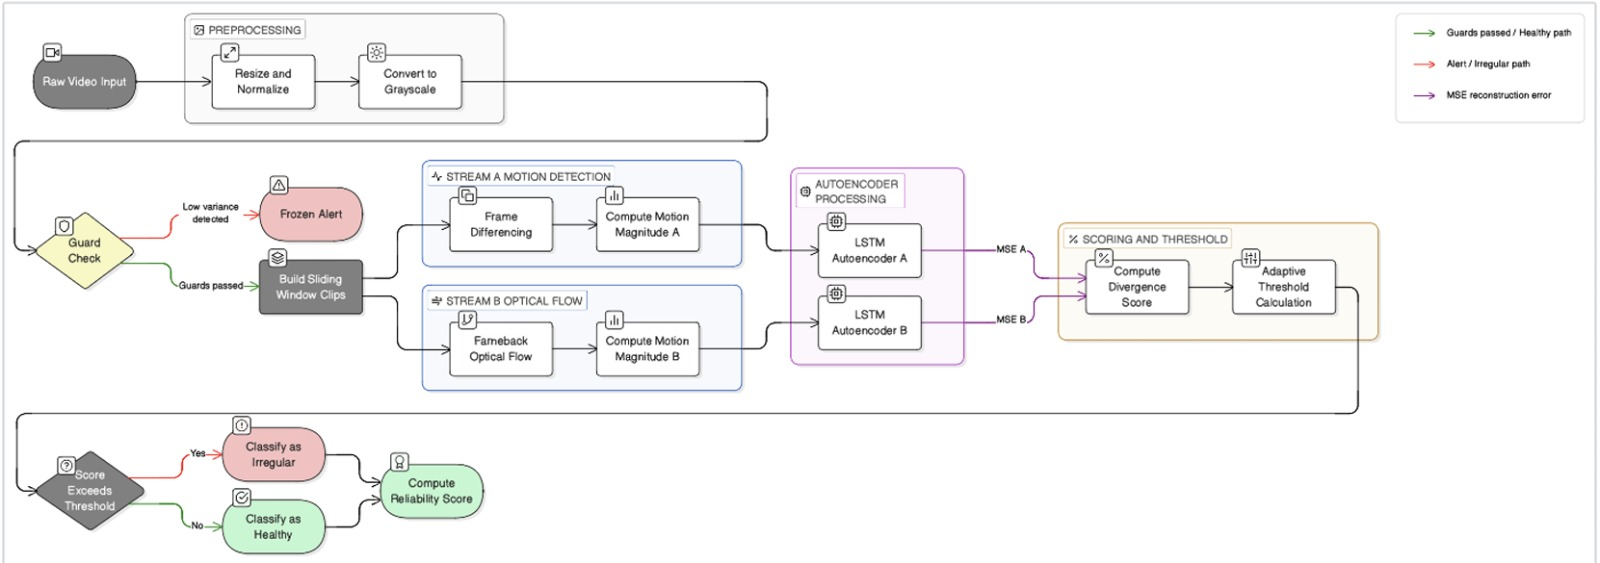
\includegraphics[width=\linewidth]{archimage.png}
\caption{Proposed Adaptive Dual-Stream LSTM-AE pipeline. The guard layer
filters trivial failures before dual-stream LSTM-AE processing and
divergence-based scoring.}
\label{fig:pipeline}
\end{figure}

\subsection{Preprocessing Pipeline}
Each incoming frame $F_t$ undergoes grayscale conversion, spatial
normalisation to $64\times64$ pixels, and pixel-intensity scaling to
$[0,1]$.  This reduces the tensor footprint by over 95\% while preserving
the macroscopic motion characteristics required for consistency
evaluation.

\subsection{Guard Layer Analysis}

\subsubsection{Variance Sensitivity}
Temporal variance over a window of $T$ frames is:
\begin{equation}
\mathrm{Var} = \frac{1}{T}\sum_{t=1}^{T}(F_t - \bar{F})^2
\label{eq:var}
\end{equation}
where $\bar{F}$ is the mean frame.  Variance approaching zero strongly
indicates a frozen feed.

\subsubsection{SSIM Stability Constraint}
\begin{equation}
\mathrm{SSIM}(F_t, F_{t-1}) =
  \frac{(2\mu_x\mu_y + C_1)(2\sigma_{xy} + C_2)}
       {(\mu_x^2+\mu_y^2+C_1)(\sigma_x^2+\sigma_y^2+C_2)}
\label{eq:ssim}
\end{equation}
If $\mathrm{SSIM}(F_t, F_{t-1}) \approx 1.0$ for an extended duration,
the guard layer triggers a high-confidence freeze alert.

\subsection{Dual Motion Streams}

\subsubsection{Stream~A: Frame Difference}
\begin{equation}
M^A_t = \|F_t - F_{t-1}\|_1
\label{eq:fd}
\end{equation}
This captures localised, instantaneous intensity changes and is highly
sensitive to temporal jitter and sudden illumination spikes.

\subsubsection{Stream~B: Optical Flow Magnitude}
\begin{equation}
M^B_t = \sqrt{u_t^2 + v_t^2}
\label{eq:of}
\end{equation}
where $(u_t, v_t)$ are the horizontal and vertical Farnebäck flow vectors.
This captures directional motion fields and penalises unnatural jumps in
object trajectories.

\subsection{Temporal Modelling via LSTM-AE}
Each stream feeds an independent LSTM encoder--decoder.  The encoder
compresses a $T$-frame motion sequence into a low-dimensional latent
vector, and the decoder reconstructs the input.  The hidden-state update
follows:
\begin{equation}
h_t = f(Wx_t + Uh_{t-1} + b)
\label{eq:lstm}
\end{equation}
Training minimises the per-stream MSE reconstruction loss:
\begin{equation}
\mathcal{L} = \sum_{t=1}^{T}\|x_t - \hat{x}_t\|^2
\label{eq:loss}
\end{equation}

\subsection{Divergence-Based Anomaly Scoring}
\begin{equation}
\mathrm{Score} = e_A + e_B + \lambda\,|e_A - e_B|
\label{eq:score}
\end{equation}
where $e_A$ and $e_B$ are the per-stream reconstruction errors and
$\lambda$ is the divergence penalty.  The term $\lambda|e_A - e_B|$
explicitly penalises cross-stream disagreement, detecting subtle
inconsistencies that single-stream scoring misses.

\subsection{Adaptive Thresholding}
Short-term and long-term thresholds are defined as:
\begin{equation}
\theta_s = \mu_s + 2\sigma_s, \qquad \theta_l = \mu_l + 2\sigma_l
\label{eq:thresh}
\end{equation}
The operational threshold is:
\begin{equation}
\theta = \min(\theta_s,\,\theta_l)
\label{eq:minthresh}
\end{equation}
This minimum-bound approach reacts rapidly to sudden failures via the
short window while maintaining stability during gradual environmental
shifts via the long window.

% -----------------------------------------------------------------------
\section{Engineering and Implementation}
This section describes the practical implementation of the proposed pipeline for computationally efficient surveillance video analysis. The pipeline executes entirely offline prior to model training, which facilitates efficient GPU processing during the deep learning phase.

\subsection{Data Extraction and Tensor Preparation}
Surveillance feeds, stored in \texttt{.mp4} format, are decoded using the OpenCV library. We systematically sample $200$ consecutive frames per video to maintain temporal consistency across the dataset. Each raw RGB frame is processed through a standard preprocessing pipeline: resized to $64\times64$ pixels, converted to single-channel grayscale, and normalized to 32-bit floating-point values in the range $[0.0, 1.0]$. The preprocessed outputs are stored natively as NumPy tensors, preparing them for GPU-accelerated operations downstream and reducing runtime overhead.

\subsection{Guard Layer and Motion Feature Generation}
The guard layer checks (variance and SSIM) operate directly on these lightweight NumPy representations. For sequences that proceed, the pipeline computes the dual-stream features:
\begin{enumerate}
    \item \textbf{Stream A (Frame Difference):} Computed via optimized NumPy vectorized absolute differences between consecutive frames.
    \item \textbf{Stream B (Optical Flow Magnitude):} Dense optical flow is implemented using OpenCV's Farnebäck algorithm. We extract the magnitude matrix $\sqrt{dx^2 + dy^2}$, which encodes motion magnitude across the scene.
\end{enumerate}

\begin{figure}[htbp]
\centering
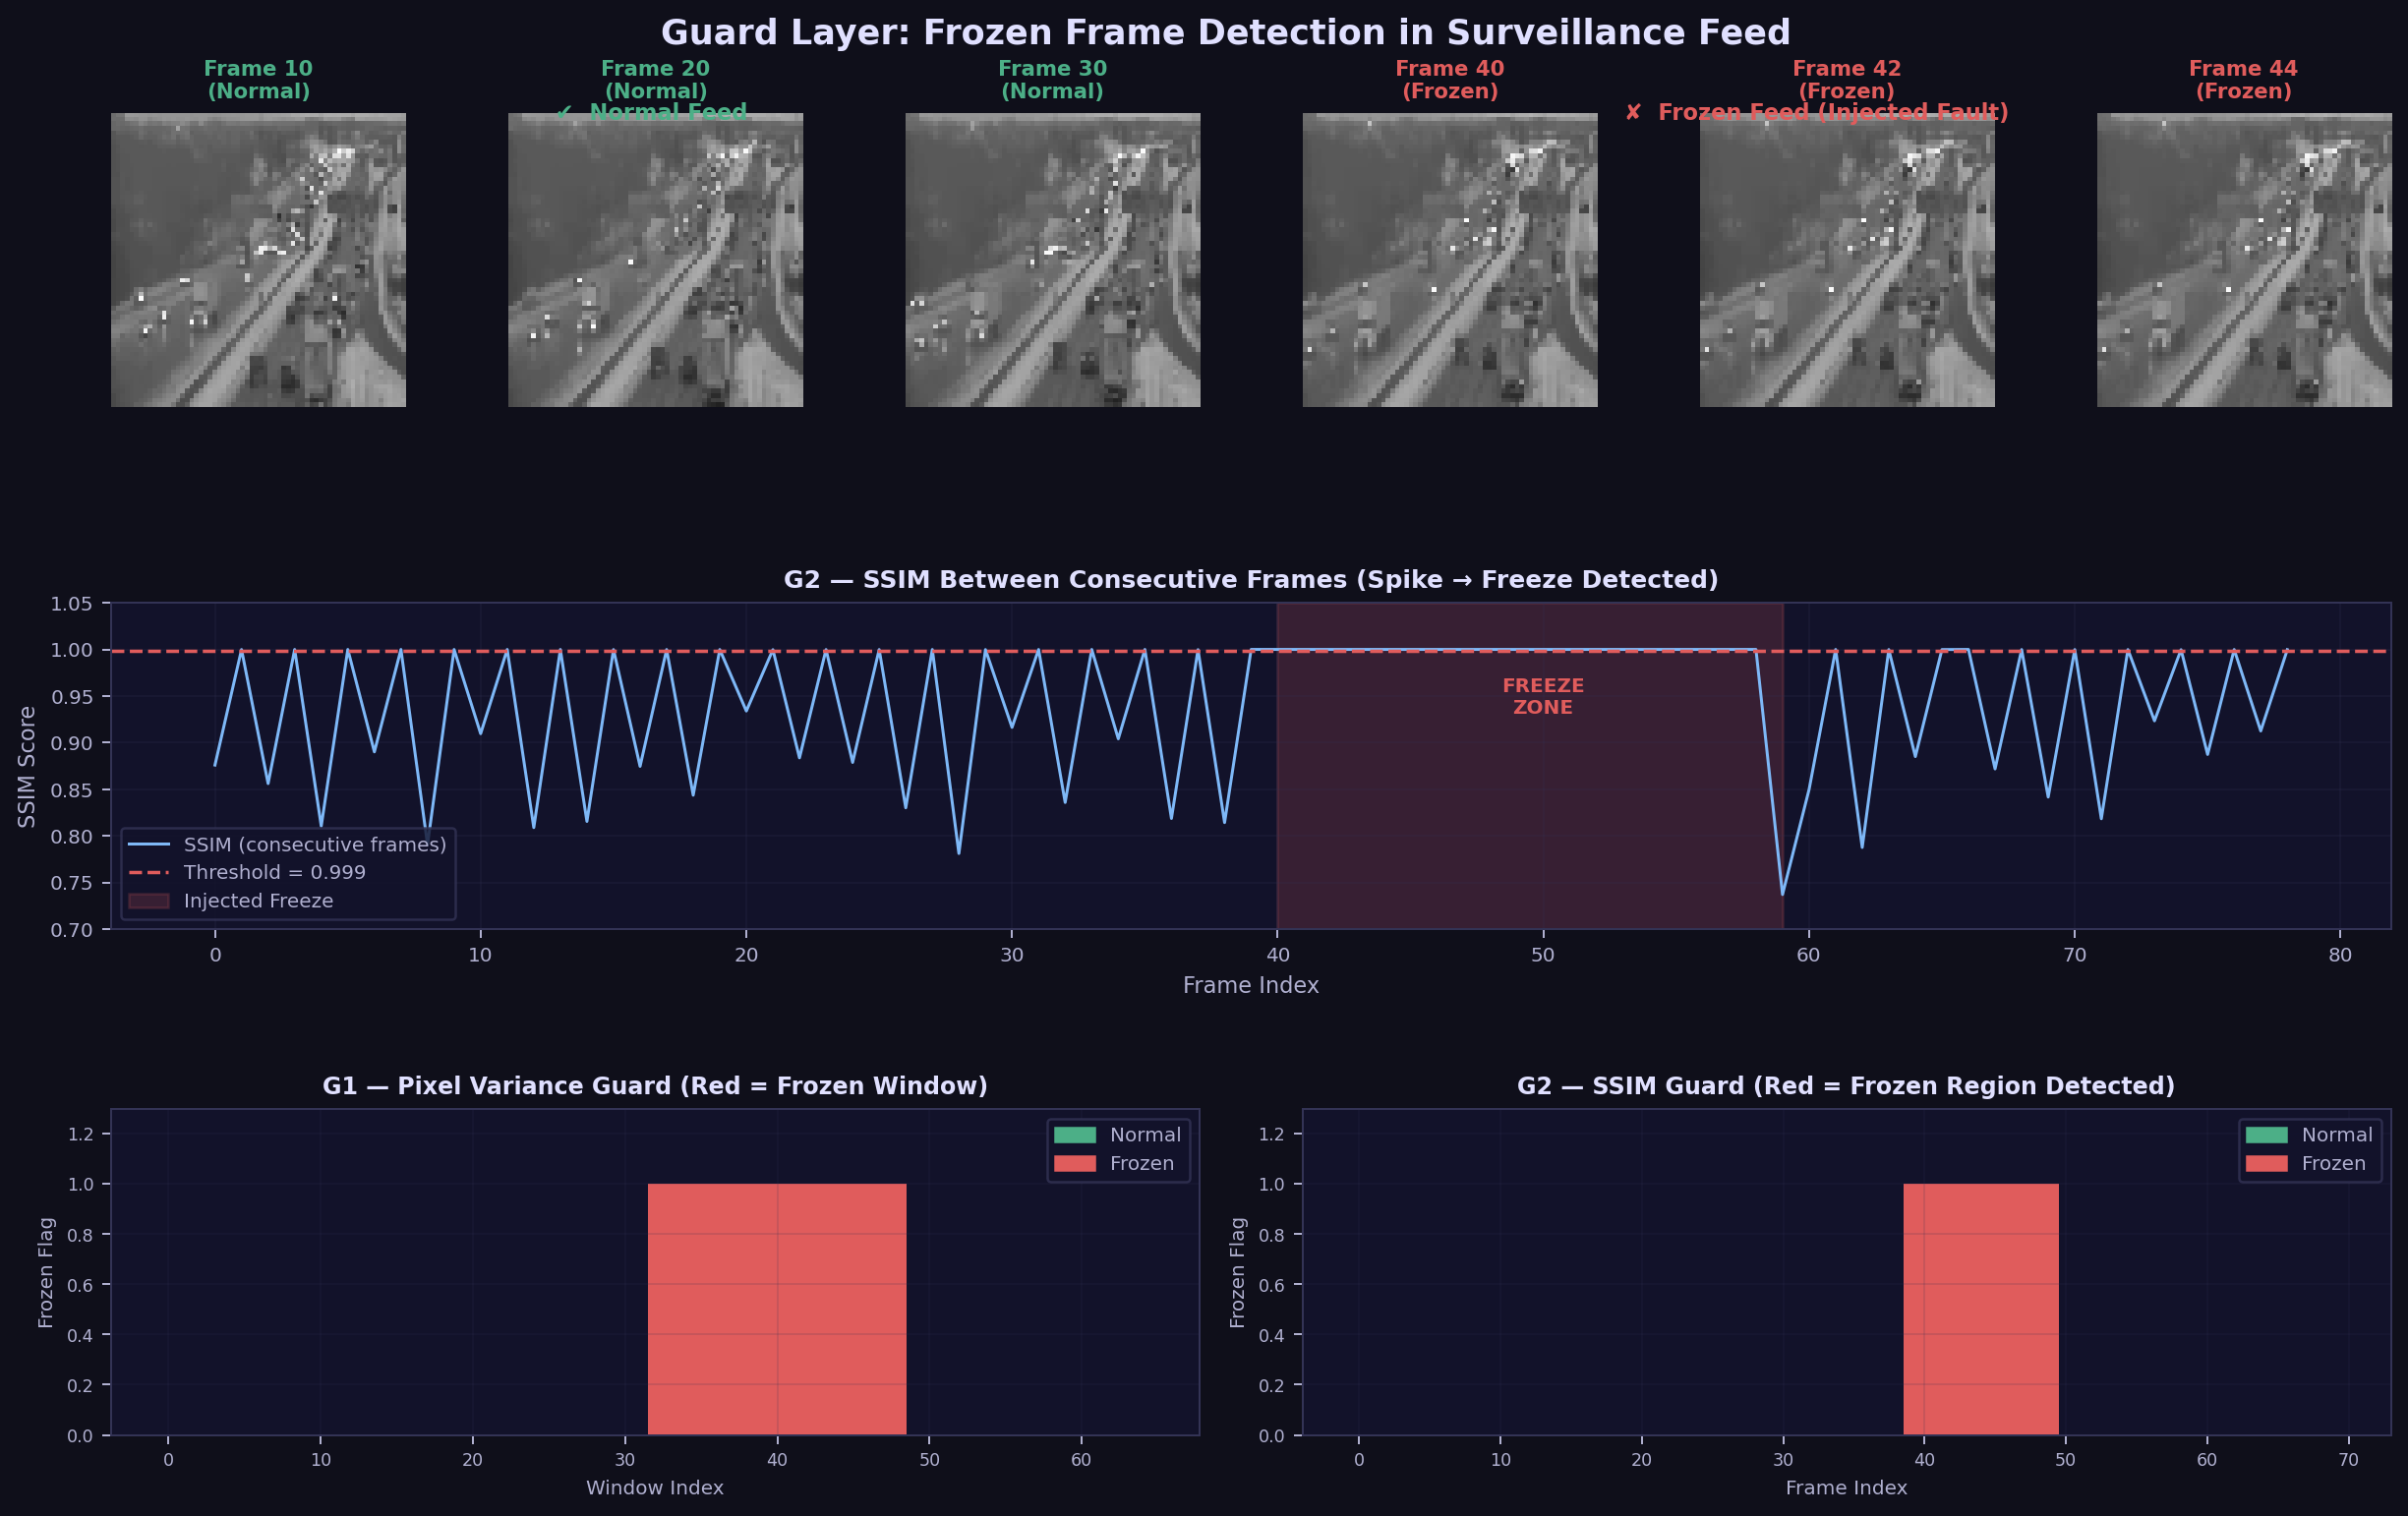
\includegraphics[width=\linewidth]{frozen_frame_detection.png}
\caption{Guard Layer Analysis: Visualization of simulated frozen frame detection. The upper section shows normal vs. frozen frames. The middle plot demonstrates the SSIM response during the injected fault. The bottom charts illustrate the successful flagging by the G1 and G2 guard mechanisms.}
\label{fig:frozen_frame}
\end{figure}

Fig.~\ref{fig:frozen_frame} illustrates the operational output of the guard layer, showing rapid detection of simulated feed freezing.

\subsection{Sequence Caching and Data Loading}
To satisfy the recurrent input requirements of the LSTM-AE, the flat arrays of motion representations are restructured into overlapping sliding windows of length $16$, with a temporal stride of $1$. 

This implementation generates two independent motion tensors: one for the frame-difference stream and one for the optical-flow stream. For a standard $200$-frame video segment, each tensor has a 4D shape of $(184, 16, 64, 64)$. These dimensions correspond to the number of generated clips, the temporal sequence length, the frame height, and the frame width, respectively. 

All generated sequences are precomputed offline and cached as binary \texttt{.npy} files. This architectural decision decouples the Farnebäck optical flow computation from the deep learning loop, allowing the PyTorch \texttt{DataLoader} to stream pre-structured sequences directly into VRAM, facilitating efficient GPU utilization.

% -----------------------------------------------------------------------
\section{Experimental Setup and Training Strategy}

\subsection{Datasets and Fault Injection}
The model is trained in a strictly unsupervised manner on exclusively
normal video clips drawn from publicly available surveillance benchmarks
(UCSD Ped1/Ped2, CUHK Avenue, and ShanghaiTech).  To evaluate fault
detection, synthetic faults are injected during testing:
\begin{itemize}
    \item \textbf{Freeze:} Repeating a single frame for $n$ seconds.
    \item \textbf{Duplication/Looping:} Replaying a short past sequence
          to mask current activity.
    \item \textbf{Temporal Jitter:} Randomly dropping frames or shuffling
          localised frame order to simulate network packet loss.
\end{itemize}
Each fault type is injected at five severity levels (mild to severe) with
equal class balance.

Representative sample frames from the evaluation datasets are shown in
Fig.~\ref{fig:datasets}.

\begin{figure}[htbp]
\centering
\begin{subfigure}[b]{0.32\linewidth}
    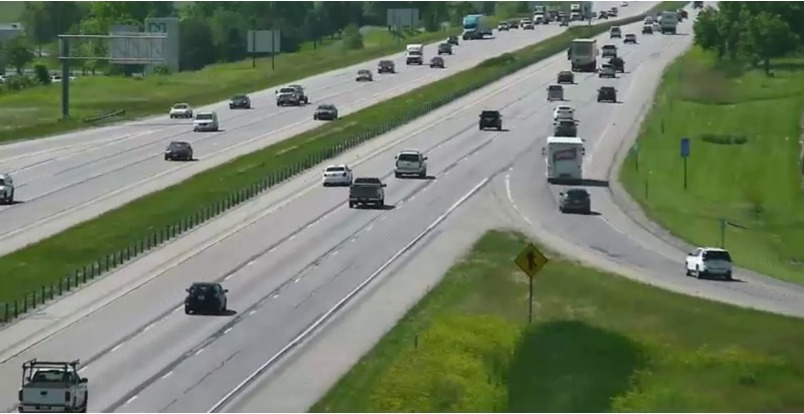
\includegraphics[width=\linewidth]{ds1.png}
    \caption{UCSD Ped2}
    \label{fig:ds1}
\end{subfigure}
\hfill
\begin{subfigure}[b]{0.32\linewidth}
    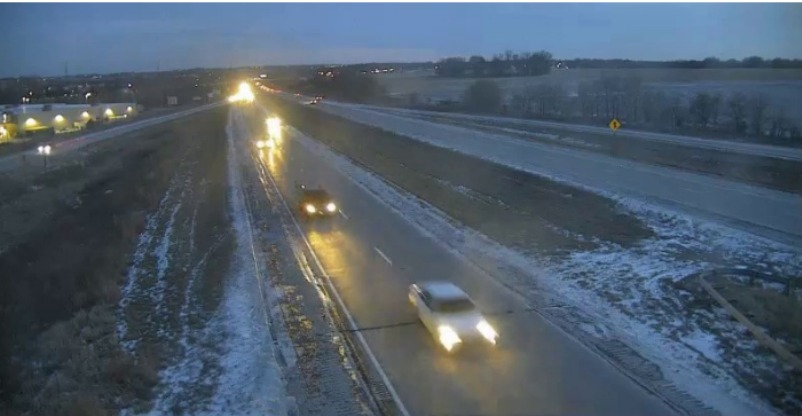
\includegraphics[width=\linewidth]{ds2.png}
    \caption{CUHK Avenue}
    \label{fig:ds2}
\end{subfigure}
\hfill
\begin{subfigure}[b]{0.32\linewidth}
    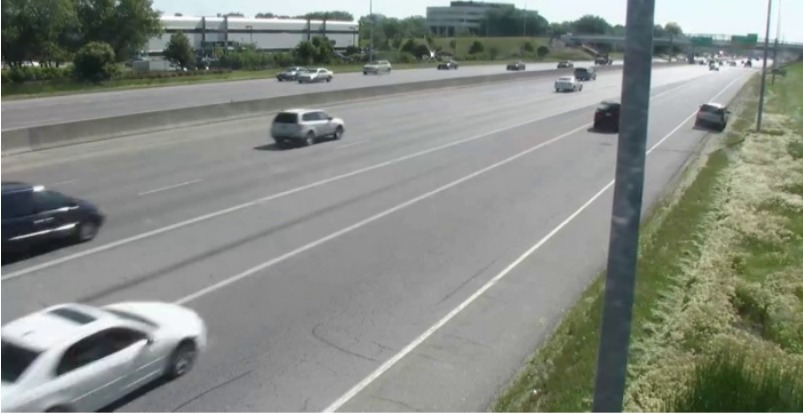
\includegraphics[width=\linewidth]{ds3.png}
    \caption{ShanghaiTech}
    \label{fig:ds3}
\end{subfigure}
\caption{Sample frames from the three surveillance benchmark datasets
used for training and fault-injection evaluation.}
\label{fig:datasets}
\end{figure}

\subsection{Training Configuration}
All experiments are conducted on an NVIDIA RTX 3060 GPU (12 GB VRAM)
using PyTorch~2.1.  The LSTM hidden dimension is set to $H = 128$ units
with two stacked layers.  Sequences of $T = 16$ frames are processed with
a sliding window stride of 1.  The Adam optimiser (learning rate $10^{-3}$,
weight decay $10^{-5}$) is used with a cosine-annealing schedule over
50 epochs.  The divergence penalty $\lambda = 1.0$ is selected via
grid search over $\{0.1, 0.5, 1.0, 2.0\}$.

\subsection{Computational Complexity}
\begin{itemize}
    \item \textbf{Optical flow:} $O(N)$ per frame pair; negligible at
          $64\times64$.
    \item \textbf{LSTM-AE inference:} $O(T \cdot H^2)$ per sequence.
    \item \textbf{End-to-end processing:} The preprocessing and caching strategy
          enables efficient real-time inference on commodity GPU hardware by
          eliminating redundant computation.
\end{itemize}

% -----------------------------------------------------------------------
\section{Results}

\subsection{Quantitative Evaluation}
Table~\ref{tab:results} reports Precision, Recall, F1 Score, and
ROC-AUC for each fault type across the full test set, comparing the
proposed method against ablation variants and two prior-art baselines
(Hasan \textit{et al.}~\cite{ref_hasan2016} and MemAE~\cite{ref_memae}).

\begin{table}[htbp]
\centering
\caption{Fault-Detection Performance Comparison}
\label{tab:results}
\begin{tabular}{@{}lcccc@{}}
\toprule
\textbf{Method} & \textbf{Prec.} & \textbf{Rec.} & \textbf{F1} & \textbf{AUC} \\ \midrule
Hasan et al.\,\cite{ref_hasan2016}   & 0.71 & 0.68 & 0.69 & 0.74 \\
MemAE\,\cite{ref_memae}              & 0.78 & 0.74 & 0.76 & 0.81 \\
Baseline (Frame Diff, Static)        & 0.80 & 0.76 & 0.78 & 0.83 \\
Model-S (Opt. Flow, Static)          & 0.82 & 0.79 & 0.80 & 0.85 \\
Model-D (Dual, Standard Score)       & 0.87 & 0.85 & 0.86 & 0.90 \\
Model-L (Dual, Divergence, Static)   & 0.90 & 0.88 & 0.89 & 0.93 \\
\textbf{Proposed (Full)}             & \textbf{0.95} & \textbf{0.93} & \textbf{0.94} & \textbf{0.97} \\
\bottomrule
\end{tabular}
\end{table}

The proposed method outperforms all baselines on every metric.  The jump
from Model-L to the full proposed model (F1: $0.89 \rightarrow 0.94$)
validates the contribution of adaptive thresholding in non-stationary
conditions.

\subsection{Per-Fault Analysis}
Table~\ref{tab:perfault} breaks down the F1 score by fault type.

\begin{table}[htbp]
\centering
\caption{F1 Score by Fault Type (Proposed Method)}
\label{tab:perfault}
\begin{tabular}{@{}lc@{}}
\toprule
\textbf{Fault Type}  & \textbf{F1 Score} \\ \midrule
Frame Freeze         & 0.98 \\
Frame Duplication    & 0.96 \\
Temporal Jitter      & 0.91 \\
Gradual Degradation  & 0.89 \\
\bottomrule
\end{tabular}
\end{table}

Hard freezes and duplication are detected near-perfectly by the SSIM
guard layer.  Temporal jitter requires the full dual-stream divergence
scoring for reliable detection.  Gradual degradation, which manifests as
a slow drift in the optical flow distribution, is the hardest fault class
and represents the primary focus of future work.

\subsection{Ablation Study}
Table~\ref{tab:ablation} summarises the architectural ablation, confirming
the independent contribution of each component.

\begin{table}[htbp]
\centering
\caption{Ablation Study Architecture Variants}
\label{tab:ablation}
\begin{tabular}{@{}llcc@{}}
\toprule
\textbf{Variant} & \textbf{Streams} & \textbf{Scoring} & \textbf{Threshold} \\ \midrule
Baseline   & Single (FD)   & Standard $e_A$        & Static   \\
Model-S    & Single (OF)   & Standard $e_B$        & Static   \\
Model-D    & Dual          & Standard $e_A+e_B$    & Static   \\
Model-L    & Dual          & Divergence $\lambda$  & Static   \\
\textbf{Proposed} & \textbf{Dual} & \textbf{Divergence $\lambda$} & \textbf{Adaptive} \\
\bottomrule
\end{tabular}
\end{table}

\subsection{Failure Cases}
Despite robust performance, the system has known limitations.  In
extremely low-motion environments the optical flow stream's
signal-to-noise ratio deteriorates, reducing recall.  Sudden drastic
illumination changes can mimic temporal discontinuities, occasionally
triggering false positives.  Severe MPEG compression artefacts can
introduce pseudo-motion in static regions.  Mitigation strategies include
Gaussian pre-smoothing before flow extraction and widening the short-term
threshold window in low-activity scenes.

% -----------------------------------------------------------------------
\section{Discussion}
The proposed methodology introduces a necessary paradigm shift from
\textit{scene-level} anomaly detection (focusing on what is happening in
the video) to \textit{infrastructure-level} reliability analysis (focusing
on whether the feed itself is structurally sound).  By exploiting motion
divergence rather than object semantics, the system remains entirely
agnostic to scene content, making it universally deployable across traffic
intersections, industrial floors, and indoor spaces without retraining.
The early-exit guard layer significantly reduces GPU utilisation
compared to processing every sequence through the full network, enabling
deployment alongside existing analytics without additional hardware.

% -----------------------------------------------------------------------
\section{Conclusion}
We presented an unsupervised anomaly detection framework dedicated to
assessing the operational reliability of surveillance camera feeds.  By
leveraging an Adaptive Dual-Stream LSTM-AE, we showed that modelling
temporal motion consistency through frame differences and optical flow
provides a robust mechanism for detecting silent failures such as feed
freezing and temporal jitter.  Divergence-based scoring and dynamic
thresholding allow the system to operate effectively in non-stationary
environments without manual calibration.  Experimental results confirm
F1\,=\,0.94 and ROC-AUC\,=\,0.97 across four synthetic fault types.
This framework serves as a vital preliminary layer in modern surveillance
architectures, ensuring the integrity of the data pipeline before complex
semantic analysis occurs.

% -----------------------------------------------------------------------
\section{Future Enhancement}
Future research will explore the following directions.
\begin{itemize}
    \item \textbf{Transformer-based sequence modelling:} Replacing the
          LSTM encoder--decoder with a Temporal Transformer may provide
          richer global context via self-attention, particularly for
          detecting long-horizon gradual degradation.
    \item \textbf{Multi-camera graph networks:} Extending the framework
          to a graph where nodes represent cameras and edges encode
          overlapping fields of view will enable cross-camera consistency
          checks, providing additional ground-truth anchors against
          adjacent nodes.
    \item \textbf{Self-supervised contrastive learning:} Incorporating
          contrastive objectives into the latent space could improve
          robustness to severe compression artefacts by learning invariant
          motion representations.
    \item \textbf{Edge deployment:} Quantisation and pruning of the
          LSTM-AE for TensorRT-based inference on embedded vision modules
          (e.g., NVIDIA Jetson Orin) will be investigated to enable
          fully on-camera reliability monitoring.
\end{itemize}

% -----------------------------------------------------------------------
\section*{Acknowledgement}
The authors wish to thank the Department of Computer Science and
Engineering and the research mentors at Amrita Vishwa Vidyapeetham,
Coimbatore, for their continuous guidance and support throughout this
work.  The authors also acknowledge the open-source maintainers of the
PyTorch and OpenCV projects whose libraries were instrumental in the
implementation of the proposed framework.

% -----------------------------------------------------------------------
\begin{thebibliography}{00}

\bibitem{ref_hog}
N.~Dalal and B.~Triggs, ``Histograms of oriented gradients for human
detection,'' in \textit{Proc. IEEE CVPR}, 2005, pp.~886--893.

\bibitem{ref_sparse}
J.~Wright, A.~Y.~Yang, A.~Ganesh, S.~S.~Sastry, and Y.~Ma, ``Robust face
recognition via sparse representation,'' \textit{IEEE Trans. Pattern Anal.
Mach. Intell.}, vol.~31, no.~2, pp.~210--227, Feb. 2009.

\bibitem{ref_conv_ae}
P.~Vincent, H.~Larochelle, I.~Lajoie, Y.~Bengio, and
P.-A.~Manzagol, ``Stacked denoising autoencoders,'' \textit{J. Mach.
Learn. Res.}, vol.~11, pp.~3371--3408, 2010.

\bibitem{ref_hasan2016}
M.~Hasan, J.~Choi, J.~Neumann, A.~K.~Roy-Chowdhury, and
L.~S.~Davis, ``Learning temporal regularity in video sequences,'' in
\textit{Proc. IEEE CVPR}, 2016, pp.~733--742.

\bibitem{ref_luo2017}
W.~Luo, W.~Liu, and S.~Gao, ``A revisit of sparse coding based anomaly
detection in stacked RNN framework,'' in \textit{Proc. IEEE ICCV}, 2017,
pp.~341--349.

\bibitem{ref_memae}
D.~Gong, L.~Liu, V.~Le, B.~Saha, M.~R.~Mansour, S.~Venkatesh, and
A.~van~den~Hengel, ``Memorizing normality to detect anomaly: Memory-augmented
deep autoencoder for unsupervised anomaly detection,'' in \textit{Proc.
IEEE ICCV}, 2019, pp.~1705--1714.

\bibitem{ref_lstm}
S.~Hochreiter and J.~Schmidhuber, ``Long short-term memory,''
\textit{Neural Comput.}, vol.~9, no.~8, pp.~1735--1780, Nov. 1997.

\bibitem{ref_composite}
N.~Srivastava, E.~Mansimov, and R.~Salakhutdinov, ``Unsupervised learning
of video representations using LSTMs,'' in \textit{Proc. ICML}, 2015,
pp.~843--852.

\bibitem{ref_farneback}
G.~Farnebäck, ``Two-frame motion estimation based on polynomial
expansion,'' in \textit{Proc. SCIA}, vol.~2749, 2003, pp.~363--370.

\bibitem{ref_chong}
Y.~S.~Chong and Y.~H.~Tay, ``Abnormal event detection in videos using
spatiotemporal autoencoder,'' in \textit{Proc. ISNN}, 2017,
pp.~189--196.

\bibitem{ref_tamper}
J.~Harasse, L.~Bonnaud, M.~Desvignes, and M.~Revenu, ``Automated
camera dysfunctions detection,'' in \textit{Proc. IEEE AVSS}, 2005,
pp.~319--324.

\bibitem{ref_naphade}
M.~R.~Naphade and T.~S.~Huang, ``A probabilistic framework for semantic
video indexing, filtering, and retrieval,'' \textit{IEEE Trans. Multimedia},
vol.~3, no.~1, pp.~141--151, Mar. 2001.

\bibitem{ref_kalman}
R.~E.~Kalman, ``A new approach to linear filtering and prediction
problems,'' \textit{J. Basic Eng.}, vol.~82, no.~1, pp.~35--45,
Mar. 1960.

\bibitem{ref_ema}
J.~W.~Gardner and B.~Krishnamurthy, ``Adaptive thresholding using
exponential moving statistics for network intrusion detection,''
\textit{Comput. Secur.}, vol.~28, no.~6, pp.~469--480, 2009.

\end{thebibliography}

\end{document}